\documentclass[14pt]{extarticle}
\usepackage{fontspec}
\usepackage{polyglossia}
\usepackage{amsmath}
\usepackage{amssymb}
\usepackage{xcolor}
\usepackage{fancyhdr}
\usepackage{graphicx}
\usepackage{listings}
\usepackage[most]{tcolorbox}
% \usepackage{setspace}
\usepackage{pifont}
\usepackage{enumitem}
\usepackage{titlesec}
\usepackage[bottom]{footmisc}
\usepackage{titling}
\usepackage{minted}
\usepackage{etoolbox}
\usepackage{array}
\usepackage{extsizes}
\usepackage{float}
\usepackage{booktabs}
\usepackage{hyperref}
\usepackage[onehalfspacing]{setspace}
\usepackage[a4paper, top=2.7cm, bottom=2.7cm, left=2.5cm, right=2.5cm, headheight=1.5cm, headsep=0.5cm]{geometry}
\usepackage{tikz}

\usetikzlibrary{automata, positioning, arrows.meta, arrows}

\newfontfamily\emoji{Segoe UI Emoji}

\pagestyle{fancy}

\setmainlanguage[numerals=western]{arabic}
\setotherlanguage{english}
% \newfontfamily\arabicfont[Script=Arabic]{Amiri}
\newfontfamily\arabicfont[Script=Arabic]{Calibri}
\newfontfamily\arabicfonttt[Script=Arabic]{Courier New}

\lstset{
  language=[Sharp]C,
  numbers=left,
  stepnumber=1,
  numbersep=8pt,
  frame=single,
  basicstyle=\ttfamily\small,
  keywordstyle=\color{blue},
  stringstyle=\color{red},
  commentstyle=\color{green!50!black}
}

\newif\ifdetailed
\ifdefined\setdetailed
  \setdetailed
\fi

\newif\ifwithsols
\ifdefined\setwithsols
  \setwithsols
\fi

% unified tcolorboxes for articles
\tcbset{colback=white, colframe=black, fonttitle=\bfseries, boxrule=0.8pt}
\newtcolorbox{boxDef}[1][]{colback=blue!5!white,colframe=blue!75!black,
  title={{\emoji📘} تعريف\ifx\\#1\\\else ~#1\fi :}}
\newtcolorbox{boxExercise}[1][]{colback=cyan!5!white,colframe=cyan!70!black,
  title={{\emoji🧩} تمرين\ifx\\#1\\\else ~#1\fi :}}
\newtcolorbox{boxExample}[1][]{colback=yellow!5!white,colframe=orange!90!black,
  title={{\emoji📝} مثال\ifx\\#1\\\else ~#1\fi :}}
\newtcolorbox{boxNote}[1][]{colback=gray!10!white,colframe=black,
  title={{\emoji✨} ملاحظة\ifx\\#1\\\else ~#1\fi :}}
\newtcolorbox{boxAttention}[1][]{colback=magenta!10!white,colframe=magenta!80!black,
  title={{\emoji🔔} تنبيه\ifx\\#1\\\else ~#1\fi :}}
\newtcolorbox{boxWarning}[1][]{colback=red!5!white,colframe=red!75!black,
  title={{\emoji⚡} ملاحظة هامة\ifx\\#1\\\else ~#1\fi :}}
\newtcolorbox{boxSolution}[1][]{colback=green!5!white,colframe=green!60!black,
  title={{\emoji✅} حل\ifx\\#1\\\else ~#1\fi :}}
\newtcolorbox{boxSymbol}[1][]{colback=purple!5!white,colframe=purple!70!black,
  title={{\emoji🔣} رمز\ifx\\#1\\\else ~#1\fi :}}
\newtcolorbox{boxHint}[1][]{colback=teal!5!white,colframe=teal!60!black,
  title={{\emoji💡} تلميح\ifx\\#1\\\else ~#1\fi :}}


\tcbset{simplecode/.style={ colback=gray!5, colframe=black!50, boxrule=0.4pt, arc=2pt, left=4pt,right=4pt,top=4pt,bottom=4pt}}
\newenvironment{boxCode}{\begin{tcolorbox}[simplecode]}{\end{tcolorbox}}

\newcolumntype{C}[1]{>{\centering\arraybackslash}p{#1}}

% redefine spaces after titles
\makeatletter
\renewcommand{\@maketitle}{%
  \begin{center}
    {\huge \bfseries \@title \par}%
    \vskip 0.2em % space between title and author
    {\large \@author \par}%
    % \vskip 0.2em % space between author and date
    % {\normalsize \@date \par}%
  \end{center}
}
\makeatother

\fancyhf{} % clear default
\fancypagestyle{plain}{
  \fancyhf{}
  \fancyhead[L]{مدرسة التسامح الشاملة}
  % \fancyhead[L]{
\includegraphics[height=1cm]{../../../images/logoTasamoh.png}}
  \fancyhead[R]{الأستاذ محمود اغبارية}
  \fancyfoot[C]{\thepage}
}

\fancyhead[L]{مدرسة التسامح الشاملة}
\fancyhead[R]{الأستاذ محمود اغبارية}
\fancyfoot[C]{\thepage}
% \date{\today}

\setcounter{tocdepth}{3} % only section subsection and subsubsection in TOC

\newcommand{\importpdfpage}[2]{%
    \thispagestyle{empty}
    \newgeometry{left=0cm,right=0cm,top=0cm,bottom=0cm}
    \includegraphics[page=#2,width=0.95\paperwidth,height=0.95\paperheight,keepaspectratio]{#1}
    \restoregeometry
}

\newcommand{\insertFullImg}[1]{%
    \noindent
    \makebox[\textwidth][c]{
        \includegraphics[width=0.9\paperwidth,keepaspectratio]{#1}%
    }%
}%

% ----------------------


% \begin{document}

% \maketitle

% % \clearpage  % start TOC on a new page
% % \renewcommand{\contentsname}{جدول المحتويات}
% % \tableofcontents
% % \clearpage

% \part*{part 1} % the * prevents numbering
% \section*{مقدمة}
% \subsection*{مثال رياضي}
% \subsubsection*{مثال فرعي}
% \paragraph*{ paragraph 1}
% \subparagraph*{sub paragraph 1}

% \ifdetailed
% \begin{english}
% \begin{minted}{csharp}
% // C# Example
% \end{minted}
% \end{english}
% \fi

% OLD WAY
% \ifdetailed
% \begin{english}
% \begin{lstlisting}
% // C# Example
% \end{lstlisting}
% \end{english}
% \fi

% % 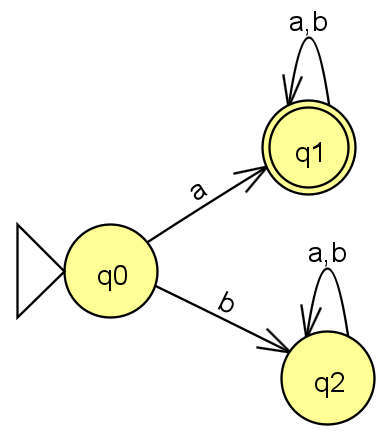
\includegraphics[width=0.2\textwidth]{../../../images/DFAs/ex1_q1.png}



% \vspace{3cm}
% \begin{flushleft}
% أرجو لكم وقتًا ممتعًا.

% الأستاذ محمود اغبارية.
% \end{flushleft}


% \end{document}


\title{تعليم جملة الشرط \textenglish{if} في \textenglish{C\#}}

\begin{document}
\maketitle

\section{المتغير المنطقي \textenglish{bool} والقيم \textenglish{True} / \textenglish{False}}

في لغة \textenglish{C\#}، النوع \textbf{\textenglish{bool}} يُستخدم لتخزين قيمتين فقط:
\begin{itemize}
    \item \textbf{\textenglish{true}} (صحيح)
    \item \textbf{\textenglish{false}} (خاطئ)
\end{itemize}

هذه القيم تُستخدم في القرارات الشرطية. مثال:

\begin{boxExample}
\begin{english}
\begin{minted}{csharp}
bool isRaining = true;
bool hasUmbrella = false;

Console.WriteLine(isRaining);   // True
Console.WriteLine(hasUmbrella); // False
\end{minted}
\end{english}
\end{boxExample}

\subsection{العمليات البوليانية (المقارنات)}

يمكننا استخدام المقارنات المنطقية لإنتاج قيم \textbf{\textenglish{bool}}:

\begin{center}
\begin{tabular}{|c|c|c|c|}
\hline
العملية & المعنى & مثال & النتيجة \\
\hline
\textenglish{>} & أكبر من & \textenglish{5 > 3} & \textenglish{true} \\
\hline
\textenglish{<} & أصغر من & \textenglish{2 < 1} & \textenglish{false} \\
\hline
\textenglish{==} & يساوي & \textenglish{4 == 4} & \textenglish{true} \\
\hline
\textenglish{!=} & لا يساوي & \textenglish{7 != 5} & \textenglish{true} \\
\hline
\textenglish{>=} & أكبر أو يساوي & \textenglish{5 >= 5} & \textenglish{true} \\
\hline
\textenglish{<=} & أصغر أو يساوي & \textenglish{3 <= 2} & \textenglish{false} \\
\hline
\end{tabular}
\end{center}

\section{جملة \textenglish{if-else} الكاملة بالأقواس}

نستخدم \textbf{\textenglish{if}} لاتخاذ قرار عندما يكون الشرط صحيحًا (\textbf{\textenglish{true}}). ويمكننا استخدام \textbf{\textenglish{else}} لتنفيذ كود آخر إذا كان الشرط خاطئًا (\textbf{\textenglish{false}}).

الصيغة العامة:
\begin{boxExample}
\begin{english}
\begin{minted}{csharp}
if (condition)
{
    // Code executed if the condition is true
}
else
{
    // Code executed if the condition is false
}
\end{minted}
\end{english}
\end{boxExample}

\begin{boxExample}
\begin{english}
\begin{minted}{csharp}
int age = 20;

if (age >= 18)
{
    Console.WriteLine("You are allowed to enter.");
}
else
{
    Console.WriteLine("You must be over 18.");
}
\end{minted}
\end{english}
\end{boxExample}

\section{يمكن حذف \textenglish{else} إذا كانت فارغة}

ليس من الضروري دائمًا استخدام \textbf{\textenglish{else}}. إذا لم يكن هناك شيء نريد فعله عندما يكون الشرط خاطئًا، يمكننا ببساطة حذفها:

\begin{boxExample}
\begin{english}
\begin{minted}{csharp}
bool isStudent = true;

if (isStudent)
{
    Console.WriteLine("Welcome, student!");
}
// No need for else here
\end{minted}
\end{english}
\end{boxExample}

\section{العمليات المنطقية \textenglish{\&\&} و \textenglish{||}}

\begin{itemize}
    \item \textbf{\textenglish{\&\&}} تعني (و): الشرطان يجب أن يكونا \textbf{صحيحين} معًا.
    \item \textbf{\textenglish{||}} تعني (أو): يكفي أن يكون \textbf{واحد} من الشرطين صحيحًا.
\end{itemize}

أمثلة:

\begin{boxExample}
\begin{english}
\begin{minted}{csharp}
bool hasTicket = true;
bool isVIP = false;

// Example of &&
if (hasTicket && isVIP)
{
    Console.WriteLine("Welcome to the VIP seat!");
}
else
{
    Console.WriteLine("Regular seat.");
}

// Example of ||
bool hasInvitation = false;

if (hasTicket || hasInvitation)
{
    Console.WriteLine("You can enter the party.");
}
else
{
    Console.WriteLine("Entry is not allowed without a ticket or invitation.");
}
\end{minted}
\end{english}
\end{boxExample}

\section{الجمل الشرطية المتداخلة (\textenglish{Nested if statements})}

يمكننا وضع \textbf{\textenglish{if}} داخل \textbf{\textenglish{if}} أخرى عندما نحتاج التحقق من أكثر من شرط بطريقة متسلسلة.

مثال:

\begin{boxExample}
\begin{english}
\begin{minted}{csharp}
int score = 85;

if (score >= 50)
{
    Console.WriteLine("Passed.");

    if (score >= 90)
    {
        Console.WriteLine("Excellent!");
    }
    else if (score >= 75)
    {
        Console.WriteLine("Very good.");
    }
    else
    {
        Console.WriteLine("Good.");
    }
}
else
{
    Console.WriteLine("Failed.");
}
\end{minted}
\end{english}
\end{boxExample}

\section{خلاصة}
\begin{itemize}
    \item \textbf{\textenglish{bool}} نوع لتخزين القيم المنطقية (\textenglish{true/false})
    \item \textbf{\textenglish{if-else}} تُستخدم لاتخاذ قرارات في الكود
    \item يمكن حذف \textbf{\textenglish{else}} إذا لم نكن بحاجة إليها
    \item نستخدم \textbf{\textenglish{\&\&}} (و) و \textbf{\textenglish{||}} (أو) للجمع بين أكثر من شرط
    \item يمكن تداخل الجمل الشرطية لمعالجة حالات متعددة بشكل متسلسل
\end{itemize}
\end{document}